% !TEX program = xelatex
% coding=utf-8
\documentclass[14pt]{Bredelebeamer}
\usepackage{ctex}

\usepackage{multirow}
\usepackage{booktabs}
\usepackage{graphicx}
\usepackage{tikz}
\usepackage{epstopdf}
\usepackage{fontawesome}
\newfontfamily{\FA}{[FontAwesome.otf]}
\usetikzlibrary{arrows,decorations.markings}
\usetikzlibrary{decorations.pathreplacing}
\usetikzlibrary{calc}
 \setbeamerfont{title}{size=\LARGE}
 \setbeamerfont{subtitle}{size=\LARGE}
 \setbeamerfont{institute}{size=\large}
%%%%%%%%%%%%%%%%%%%%%%%%%%%%%%%%%%%%%%%%%%%%%%%%



\title[研究生开题答辩]{神经网络语言模型的性能优化研究}
\subtitle{On Optimization Perspective of Neural Language Model}
\institute[]{北京航空航天大学计算机学院研究生开题答辩}
\author[\href{mailto:nanjiang@buaa.edu.cn}{ \textit{nanjiang@buaa.edu.cn}}]{姜楠 (\href{mailto:nanjiang@buaa.edu.cn}{\textit{nanjiang@buaa.edu.cn}})}
\date{ 2016 年 12 月 20 日}
\subject{开题答辩}

\begin{document}

\begin{frame}
  \titlepage
\end{frame}

\begin{frame}{概览}
  \begin{columns}
    \begin{column}{.5\textwidth}
        \tableofcontents
    \end{column}
    \begin{column}{.5\textwidth}
      \begin{figure}
        \centering
        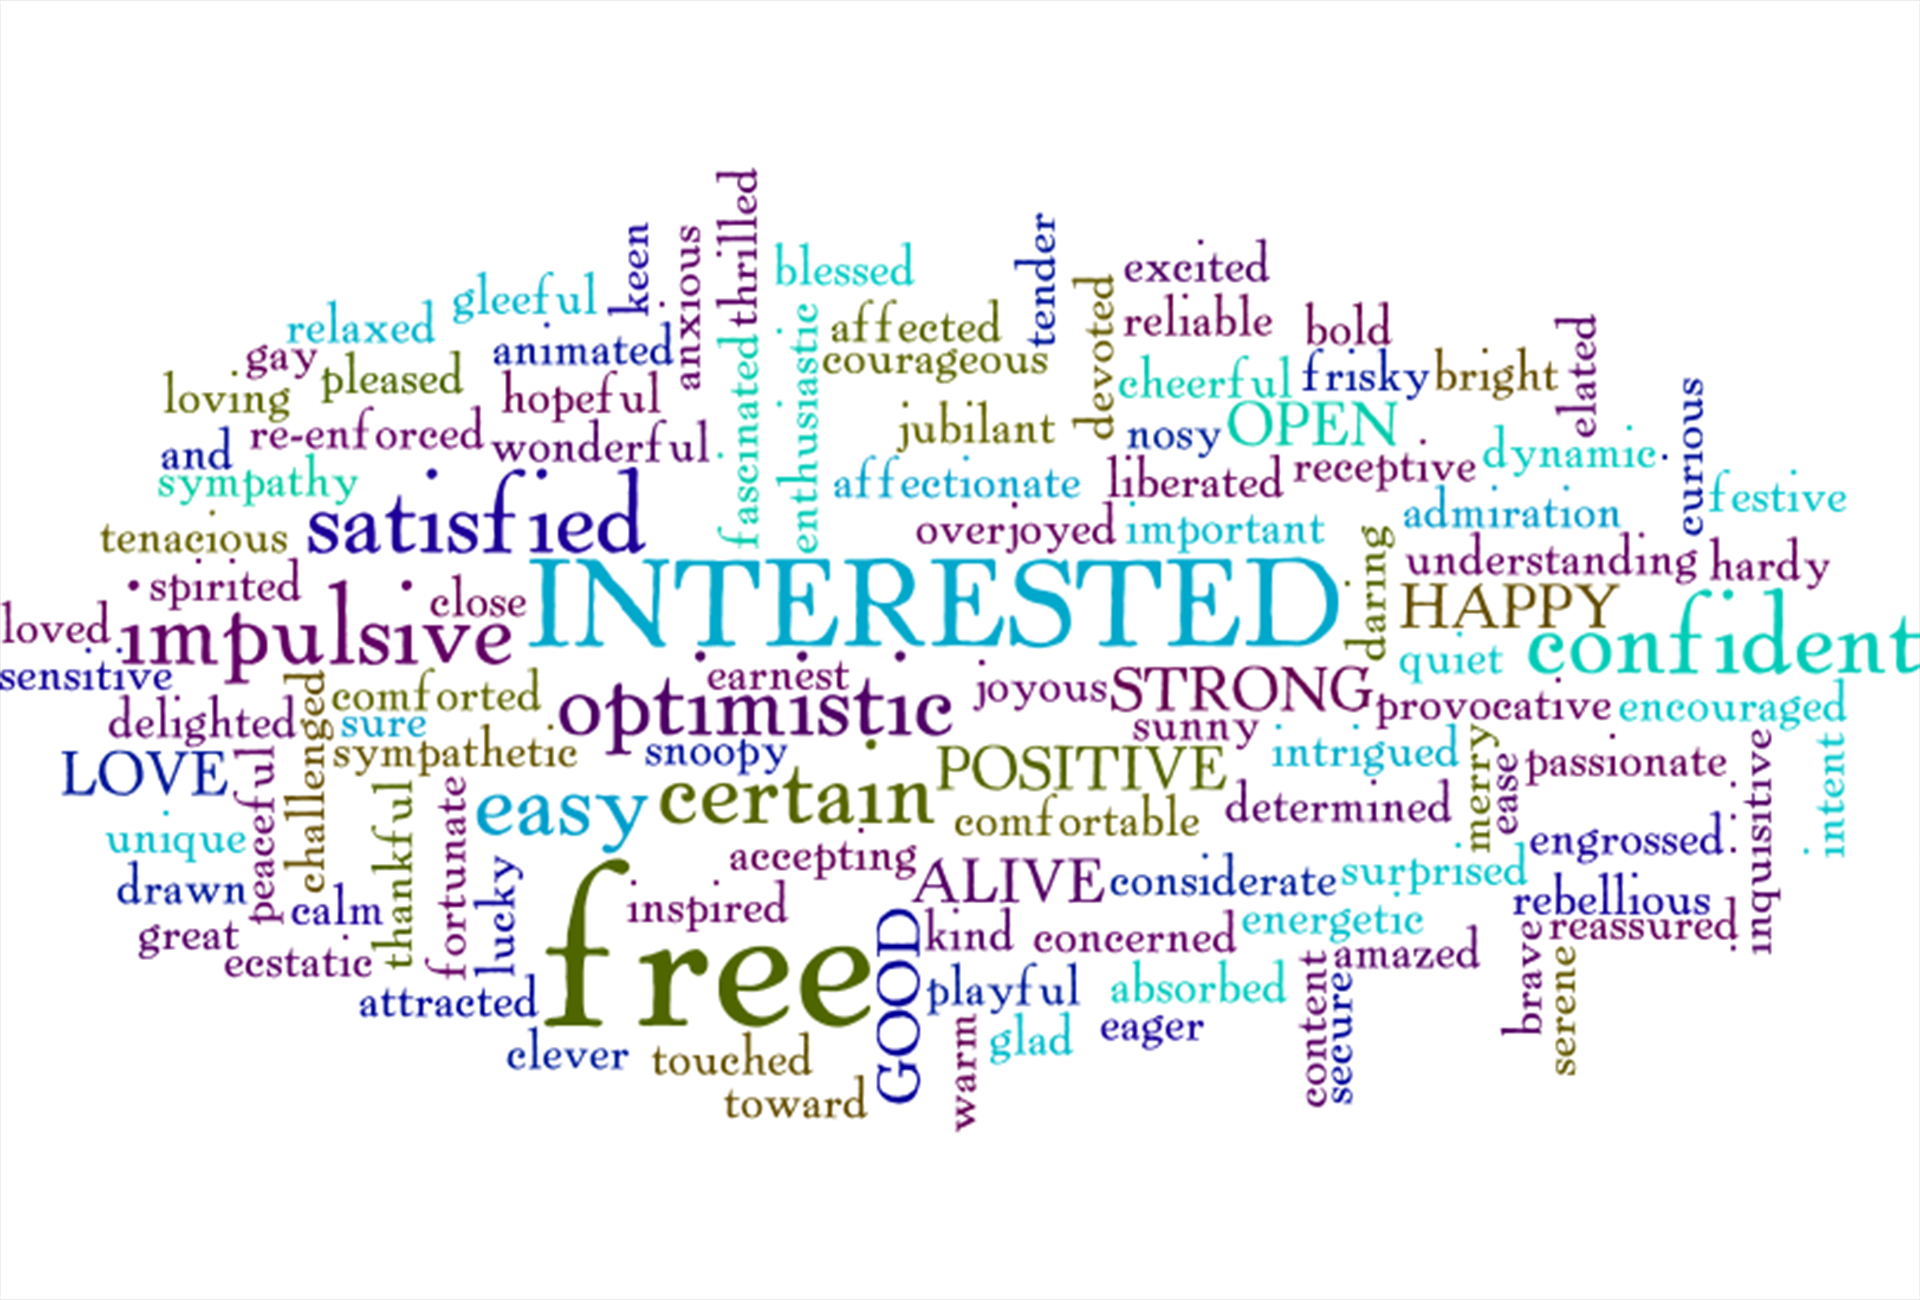
\includegraphics[width=1.\textwidth]{images/word-cloud.png}
      \end{figure}
    \end{column}
  \end{columns}
\end{frame}

\section{论文选题的背景与意义}
\begin{frame}{题目来源}
  论文题目《神经网络语言模型的性能优化研究》为自拟课题。
  \pause
  \begin{alertblock}{LSB隐写术(LSB Steganography)}
    \begin{itemize}
      \item 最早接触隐写术的概念在《密码学》课堂上
      \item 因为感兴趣曾经使用Wolfram Mathematica实现了基本的隐写程序,并写入了博客
    \end{itemize}
  \end{alertblock}
  \pause
  \begin{block}<3->{支持向量机(SVM)}
    \begin{itemize}
      \item 机器学习是现在非常流行的研究方向,可以在很多领域实现优化
      \item 完成过SVM相关的实战
    \end{itemize}
  \end{block}
  \pause
  所以在毕设中尝试完成应用SVM针对LSB图像隐写进行优化。
\end{frame}

\section{国内外研究现状及发展动态}
\begin{frame}{语言模型}

{\large
隐写是指把一个文件、消息、图像或者视频隐藏到另一个文件、消息、图像或者视频的行为。与密码学不同的是,隐写术旨在隐藏消息或其他形式的信息本身的\alert{存在},不引起发送方和接收方以外的人的怀疑而完成信息的交流,而密码学则用于隐藏这些信息的\alert{内容},使得非发送方或接收方即使截获消息也无法得到所交流的信息的真实内容。
必须满足条件:
\pause
\begin{itemize}
  \item	保密性
  \item 可获得性
  \item 完整性
\end{itemize}
}
\end{frame}


\subsection{隐写分析}

\begin{frame}{隐写分析}
  \begin{columns}
    \begin{column}{.25\textwidth}
      \begin{block}{}
        \begin{itemize}
          \item \alert<2>{视觉隐写分析}
          \item 结构隐写分析
          \item 统计隐写分析
          \item 学习隐写分析
        \end{itemize}
      \end{block}
    \end{column}
    \begin{column}{.7\textwidth}
      \pause
      \begin{figure}
        \centering
        \includegraphics[width=.95\textwidth]{images/lsb1}
      \end{figure}
    \end{column}
  \end{columns}
\end{frame}












\section{论文的研究内容及拟采取的技术方案}



\begin{frame}{循环神经网络}
	\begin{block}{样本集}
		容量为$N$的训练样本集$D = \left\{ {\left( {{{\mathbf{x}}_1},{y_1}} \right),\left( {{{\mathbf{x}}_2},{y_2}} \right), \ldots \left( {{{\mathbf{x}}_N},{y_N}} \right)} \right\}$
    \pause
		\begin{itemize}
			\item 特征向量${\mathbf{x}_i}$为图像块的特征
      \pause
			\item 标签$y_i \in \left\{ -1,1\right\}$为安全评估结果,在训练集中由隐写方法评估得到,在使用隐写系统时预测结果作为选择位置的参考指标
		\end{itemize}
	\end{block}
\pause
	\begin{alertblock}{SVM分类器}
			\begin{columns}
			\begin{column}{.5\textwidth}
		追求最大\alert<4>{“间隔”}的分类
		$$
		\begin{aligned}
		\mathop {\max }\limits_{{\mathbf{w}},b} & \quad\frac{2}{{\left\| {\alert<4>{\mathbf{w}}} \right\|}} \\
		s.t. &\quad {y_i}  \left( {{{\mathbf{w}}^T}{\mathbf{x_i}} + b} \right) \ge 1,i = 1,2, \ldots ,N
		\end{aligned}$$
			\end{column}
      \pause
					\begin{column}{.41\textwidth}
						过度拟合\&线性不可分
						\begin{itemize}
              \pause
							\item 核函数:变换特征空间至高维
              \pause
							\item 软间隔:以权重$C$容忍分类错误
						\end{itemize}
						\end{column}
		\end{columns}
	\end{alertblock}
\end{frame}






\subsection{拟采取的技术方案}
\begin{frame}{实验平台和设置}
	\begin{description}
		\item[Linux] 操作系统
		\item[R] 主要用于数据统计和图表处理
		\item[Python2.7] 使用的开发语言和开发环境
		\item[Theano] 主要的建模语言
	\end{description}
  \pause
	\begin{block}{}
		\begin{itemize}
			\item 同时还依赖于其他的处理脚本,需要对bash script和C/C++ 有足够的了解和掌握;
			\item GPU的设备是使用Titan X, 并且对应的CUDA版本为8.0(需要CUDNN/CUSPARSE等库的支持).
		\end{itemize}
	\end{block}
\end{frame}

\subsection{论文的研究内容}
\begin{frame}{SVM的训练}
	使用80组不同参数进行训练,得到的SVM在错误率方面的表现
\end{frame}

\section{论文研究计划}
\begin{frame}{时间安排}
	\begin{block}{}
\begin{itemize}
  \item 2016年12月 $\sim$ 2017年1月: 整理资料,学习研究语言模型的领域知识;
  \item 2017年2月$\sim$ 2017年4月: 研究学习深度学习模型的知识, 特别是循环神经网络的建模过程;
  \item 2017年5月$\sim$2017年7月: 调研并实现解决大词表问题的主要手段, 并实现基本代码框架;
  \item 2015年8月$\sim$2015年10月: 实验验证与完善;
  \item 2015年11月$\sim$2015年12月:资料整理和论文撰写.
\end{itemize}
    \end{block}
\end{frame}

\begin{frame}{Thanks}
	\centering
    谢谢各位老师和同学!请大家批评指正;

	论文中用到的全部源代码(包括本幻灯片),数据,图像,文档见:
	 {\faGithub~~\url{https://github.com/jiangnanHugo/Graduate_Design}}
\end{frame}

\end{document}
